\chapter{State of the Art} % Main chapter title
\label{chap:StateOfTheArt}
Developing a platform that supports multiple types of services and with the ability to grow in terms of both features and traffic, requires it to be built with the best quality standards of software engineering. In this chapter, we will firstly analyze approaches of other platforms already on the market, and present the state of the art on software architecture, by researching on several architectural designs that might be applicable to this project.

\section{Existing Solutions}
In this section will be presented some existing solutions that have similar requirements to this project. The analysis of these platforms will help to understand what problems may arise, and how these companies tackled them.

\subsection{UberEats}
With the success that Uber was having in the passenger transportation sector, in 2014, the company started on the food delivery business. Initially, this was a side project that was integrated Uber's main app. The service was only available for lunch, and number of options were scarce. Note that this occurred in a time where there were already other competitors offering food delivery services, without these restrictions \parencite{whyUberStartedUberEats}. 
\par
UberEats is a food delivery service offered by Uber, that connects several restaurants to the customers in the restaurant's surrounding area. Contrary to what the competition was doing, UberEats limited the access to place orders to customers in zones where there were restaurants in their network \parencite{whyUberStartedUberEats}. This decision allowed three things: first, to increase the quality. It is impossible to keep the quality of a product after it had to go through several kilometers in order to be delivered to the customer. Second, it diminished the delivery time. People want to be able to order food minutes before lunch/dinner time. By limiting the areas where it was available, it was also possible to increase speed time. Last, but not the least, it enabled to keep a low, flat rate for all delivery services.
\par
Uber, and by consequence UberEats, is a company that was, since the beginning, very mobile oriented. Mobile e-commerce has grown a lot in the last ten years. In fact, since 2017, it counts for over half of the whole web traffic \parencite{percentageMobileTraffic}. The rise of the smartphones and with telecommunication companies offering better and cheaper services was a key fact that enabled this rise in the mobile share. This behavior is even more noticeable when the data relative to e-commerce is analyzed. The graph in figure \ref{fig:mobileGrowth} refers to the growth of the market share for mobile e-commerce\footnote{data retrieved from https://hostingfacts.com/internet-facts-stats/}. In 2018, the market share for mobile e-commerce was 63.5\%, and it is expected to grow as high as 72.9\% until 2021.

\begin{figure}[ht]
\centering
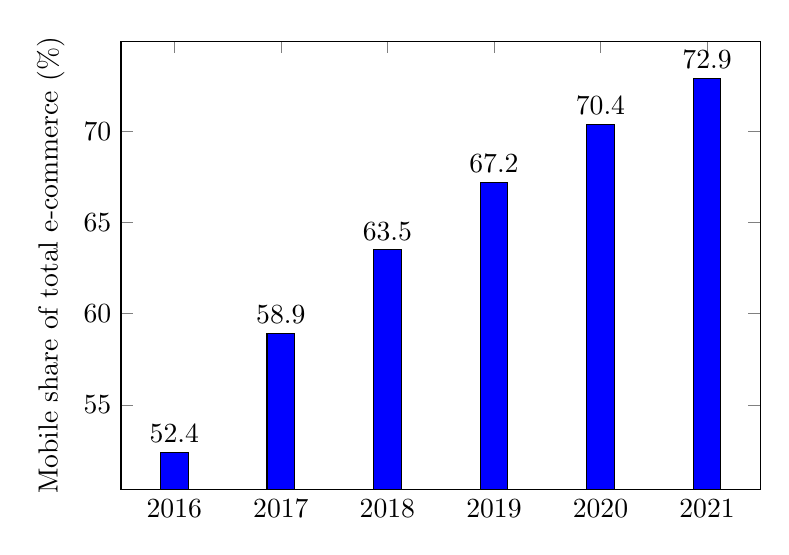
\begin{tikzpicture}
        \begin{axis}[
            symbolic x coords={2016, 2017, 2018, 2019, 2020, 2021},
            ylabel=Mobile share of total e-commerce (\%),
            width=0.8\textwidth,
            height=0.6\textwidth,
            nodes near coords,
            nodes near coords align={vertical},
          ]
            \addplot[ybar,fill=blue] coordinates {
                (2016,  52.4)
                (2017,  58.9)
                (2018,  63.5)
                (2019,  67.2)
                (2020,  70.4)
                (2021,  72.9)
            };
        \end{axis}
    \end{tikzpicture}
\caption{Mobile share of total e-commerce 2016 to 2021}
\label{fig:mobileGrowth}
\end{figure}

This means that Uber was right on the start of the mobile trend, when it started, which was a very positive factor when evaluating the growth of their business.

\subsection{Glovo}

Glovo started in 2015 with a business model similar to UberEats. However, the two companies differed on what products they delivered. While UberEats is focused on food delivery, Glovo has a broader range of products that they are able to deliver. According to Glovo's website, they are able to deliver "food, gifts, markets, pharmacy, snacks \& juices, anything". As the company advertises, in addition to the services that they provide (ordering food, medicine...), the platform is also able to process and deliver miscellaneous items, defined by the customer. 
\par
Despite the possibility for the customer to order almost anything on Glovo, the most used service is, actually the food delivery. This makes Glovo a competitor to Uber Eats which customers choose, typically, based on price and delivery time. Glovo also offers certain options that are not available in UberEats. An example of that is the possibility to add instructions of how well done the meat is wanted. On the other hand, UberEats provides an estimated delivery time, while Glovo only offers abstract information about the status (for example, "your Glovo is being collected") \parencite{uberVsGlovo}.
\par
Similarly, the approach was unsurprisingly very mobile driven, since when the company started, the mobile phenomenon was already very prominent. Nevertheless, taking into account the figure \ref{fig:mobileGrowth}, it was a good decision, since the mobile share on total e-commerce keeps growing.

\section{Technology}
\label{sec:StateOfTheArt_Technology}
In this section the current state of the art in terms of technology will be analyzed. Architecture and developing frameworks are the topics that will be discussed in the next pages. The research done for these topics is essential to fully understand the pros and cons of each approach, and how they fit (or not) this project.

\subsection{Architecture}
\label{sub:StateOfTheArt_Technology_Architecture}
As it is in the software development life cycle, the first topic that will be tackled is the architecture. This research will help the understanding of the best practices in terms of software design, and which approaches are a better fit for this project.
\par
Architecture can be defined as the structure of the various components within a system, how the communicate with each other, the constraints, principles and guidelines. It must be taken into account that these last three points are dynamic and often change over the time \parencite{mappingServicesToActivities}. In the next few sections, the architectural styles \gls{SOA}, Micro-Services, and \gls{CQRS} will be presented.

\subsubsection{Service Oriented Architecture}
\gls{SOA} is an architectural style that has as its main purposes, the focus on the business, modularity and reuse. It consists in splitting the system's functions into small applications, each one representing a real business activity. That business activity is what is called a service. The services that exist in a system must provide an interface in order to communicate with other services.
\par

The systems that follow this architecture may be called service-oriented applications. These applications typically follow an architecture similar to the one presented in figure \ref{fig:soaExample}. 
\par
\begin{figure}[ht]
\centering
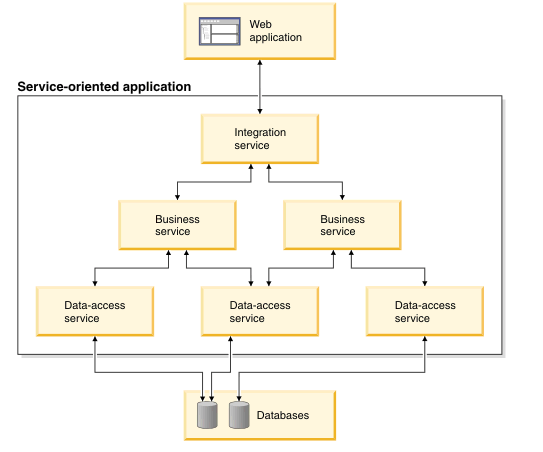
\includegraphics[width=0.8\textwidth,keepaspectratio]{chapters/State_of_the_Art/assets/soa_arch.png}
\caption[Service Oriented Architecture Example]{Service Oriented Architecture Example\footnotemark}
\label{fig:soaExample}
\end{figure}
\footnotetext{retrieved from \url{https://www.ibm.com/support/knowledgecenter/en/SSMQ79_9.5.1/com.ibm.egl.pg.doc/topics/pegl_serv_overview.html}}


\par
This architectural style is one of the most common on companies. In fact, "it has become the excellent methodology of system construction" \parencite{soaPetroleum}.
\par
The architecture is composed of three main blocks. The topmost level is where are the responsible for the integration of the application with external services/applications. This is often accomplished with an \gls{ESB}. An \gls{ESB} is communication system that abstracts the conversion of different protocols into a single component. This layer communicates with the business services. The business services are located in the second layer of the application and processes low-level business operations. The business logic inherent to the system, would be implemented in this layer. The integration layer will call several business services in order to process a business operation. Taking the e-commerce example, when processing an order, the business services could be fetching the information of the product, calculate order values and process invoice. Lastly, the third level of the architecture consists of data-access services, responsible to retrieve and persist information in the database. The business services use this layer in order to have access to the information and then return it, when processed, to the integration layer. It may also happen the other way around. For create/update operations, when the integration service passes information onto the business services, that information will be processed and sent to the data-access layer, where it will be persisted in the database. In addition to databases, it may also access message queues to send events \parencite{soaIBM}.


\par
\gls{SOA} has many variations and extensions, applying new patterns and good practices adapted to new realities. Micro-Services is one of them.

\subsubsection{Micro-Services Architecture}
\label{sub:StateOfTheArt_Architectures_microservices}
Micro-Services, or Micro-Services Architecture, are a part of \gls{SOA} where the services are more fine grained. These services should be independent of each other in order to be as loosely coupled as possible. Micro-Services Architecture is widely known for following the \gls{SRP}, since its function within the system is very well defined.
\par
This approach is perfect for complex systems, given that they are typically heterogeneous, unbounded and dynamic. The architecture of these systems must employ a high level of abstractions, to be able to deal with the complexity of these systems. 
\par
A service that consumes another, doesn't need to know any internal logic of it, as long as a clear interface has been defined. The interface is what is responsible for the establishment of a contract that enables a consumer to be able to communicate. Each of these services must be autonomous. This means that, as long as none of the contracts has been broken, each service is responsible for itself. For example, in a product service, that has as its main responsibility, the management of the products on an e-commerce platform. As far as the contracts established are not broken (no longer be able to create products in the same way, is a good example of this), the service may change the way it manages the products. This also means that consumers must be abstracted of how, in this case the product service, works internally and just use the contracts, as a service.
\par

\begin{figure}[ht]
\centering
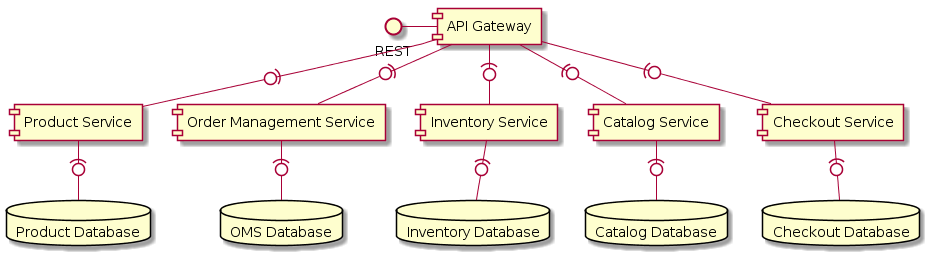
\includegraphics[width=\textwidth,keepaspectratio]{chapters/State_of_the_Art/assets/SOA_example.png}
\caption[Microservices Architecture Example]{Microservices Architecture Example}
\label{fig:microservicesExample}
\end{figure}

\par
In figure \ref{fig:microservicesExample} is presented an architectural example of micro-services. This example follows the one previously mentioned of an e-commerce platform. In the figure, it is possible to verify that the responsibilities are divided into five services:
\begin{itemize}
  \item \textbf{Product Service}, with the responsibility of managing the existing products on the platform;
  \item \textbf{Order Management Service}, which is responsible for processing the orders;
  \item \textbf{Inventory Service}, is who is responsible for managing the quantity of each product that is available;
  \item \textbf{Catalog Service}, managing which products are available and when;
  \item \textbf{Checkout Service}, with the responsibility of finishing the order on a front-office side and process the payment.
\end{itemize}

\par 
As it was mentioned, these services are completely loosely coupled since there are no dependencies between any of them. Every service is also entitled and responsible for maintaining its own database, where it will store the data necessary to its correct functioning. In a well implemented micro services architecture, it should also be possible to deploy each of the services independently, without impacting the correct functioning of the others.


\subsubsection{Command Query Responsibility Segregation}
\label{sub:StateOfTheArt_Architecture_CQRS}
\gls{CQRS} is a pattern described by Greg Young where it is defended that the models used to update information and the models used to read information can be different \parencite{cqrs}. The most common use of a database is often a \gls{CRUD} approach. This means that all create, read, update and delete operations use the same model. This approach often brings some disadvantages. It can turn the management of permissions and security into a more complex task, since each entity is target of both read and write operations. It may also lead to an information mismatch since some fields may not be required some information that is already existent in the database. Finally, it may create concurrency problems, when a set of services operate over a given amount of data. This might also create performance issues, since read and write operations can't be scaled independently \parencite{microsoftCqrs}.
\par

This separation maps directly with the command and query concept. Write operations, like \gls{CRUD}'s create, update and delete actions, are commands. Read operations that solely retrieve information are considered queries.
\par
This pattern separates these two operations by having two different interfaces. By doing this, the possibility of having different models is also enabled. On the other hand, \gls{CQRS} can't be automatically generated by scaffold mechanisms as \gls{CRUD} can \parencite{microsoftCqrs}. \gls{CQRS} is often implemented by having two different services, one responsible for the queries, other responsible for the commands. This allows to scale the system independently, which can be useful on services that have a high load of reads, but not many updates.

\par 

\gls{CQRS} is recommended to be used only in specific parts of a system. In particular, parts where there is a high chance of concurrence and/or parts where \gls{DDD} was used. It is also a good option for systems that need to handle high performance applications, because, not only as said earlier, it is possible to scale independently, but also because is possible to add different optimization to each side \parencite{cqrs}.
\par

In the figure \ref{fig:cqrsExample}  there is a schema of a typical \gls{CQRS} implementation. It is possible to see the two interfaces that are available, one for the queries, and other for the commands. In case of the command, the interface is connected to its model where it will validate the user/consumer's input and, then, proceed to the operation in the database. For the queries, the behaviour is very similar. After the user/consumer's request, it is sent to the model, which then retrieves the data from the database and processes it. Finally, the information is returned to the requester.

\par

\begin{figure}[t]
\centering
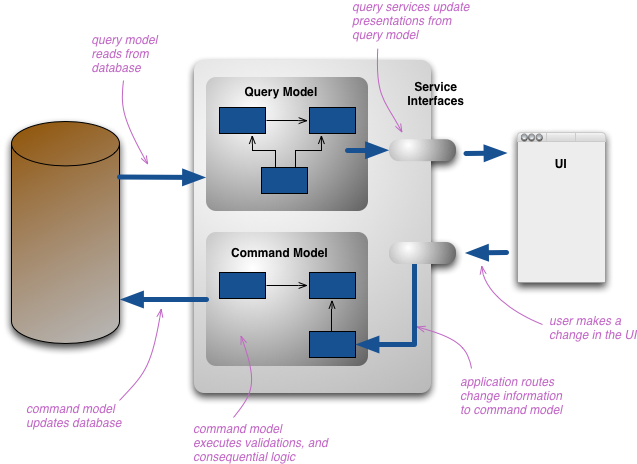
\includegraphics[width=0.8\textwidth,keepaspectratio]{chapters/State_of_the_Art/assets/cqrs.png}
\caption[CQRS Typical Implementation]{CQRS Typical Implementation\footnotemark}
\label{fig:cqrsExample}
\end{figure}
\footnotetext{retrieved from https://martinfowler.com/bliki/CQRS.html}
\par

\gls{CQRS} is a very powerful architecture that solves many specific problems. However, before deciding to use this pattern, a careful analysis should be carried out. The implementation of this pattern requires a change in mindset and many information systems fit in the traditional approach, and implementing \gls{CQRS} would add unnecessary complexity to the project \parencite{cqrs}.

\subsubsection{Event Sourcing}
\label{sub:StateOfTheArt_Architecture_EventSourcing}
Event sourcing is an architectural style, where every change in the state of an entity triggers an event, and that the event is stored in the same sequence that they were applied. The whole purpose of doing this is to replicate the state of a certain entity by reprocessing all the events \parencite{martinFowlerEventSourcing}.

\par
This architecture also passes the responsibility of calling all operations inherent to a business process to the services that actually do that operations. In contrary to \gls{HTTP} calls, where the source (which triggers the event) needs to know processes to call, in event sourcing (and most event-driven architectures), the source only needs to make sure that the event is published. The listeners are the ones who need to check if that particular event is something that needs to start any operation
\par
The figure \ref{fig:kafkaEvent} presents an example for this situation. The user sends a request to the front-end server, which then publishes an event to the Kafka Broker. When this happens, both "First Service" and "Second Service" will receive the information about what happened, and then decide if they should trigger any process regarding the user action.

\begin{figure}[ht]
\centering
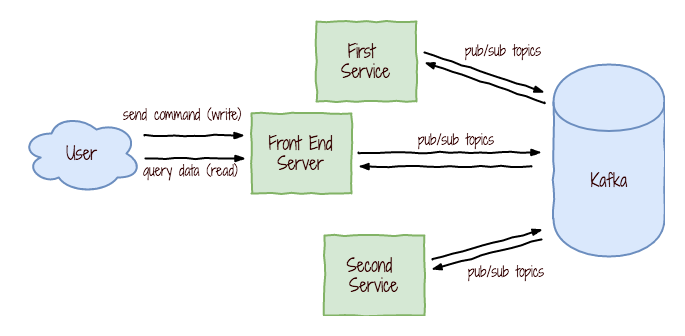
\includegraphics[width=0.8\textwidth,keepaspectratio]{chapters/State_of_the_Art/assets/kafka-event-sourcing.png}
\caption[Event Driven Architecture using Kafka]{Event Driven Architecture using Kafka\footnotemark}
\label{fig:kafkaEvent}
\end{figure}
\footnotetext{retrieved from \url{https://medium.com/kontenainc/event-sourcing-microservices-with-kafka-2568801527d8}}


\par

This architecture is very good for any application that needs to keep track of every change that occurred on a certain entity of their business. Bank systems are a good example where this architecture may be used. There must be a record of every transaction that is made in a bank account and with event sourcing, that is done, and the events produced will trigger the necessary processes to run. 

\subsection{Software Development Frameworks}

In this section, an overview will be given over the current most used software frameworks. These frameworks are used as abstractions over more specific \gls{OS} code, thus enabling its re-use. Furthermore, they provide several libraries, tools and compilers to facilitate the developer's work. Currently, the use of these abstractions is a standard to build and deploy applications within the industry. In the next sections, we will analyze the frameworks .NET Core, Java Spring and Node.js.

\subsubsection{.NET Core}
\label{sub:StateOfTheArt_Frameworks_NET}
.NET is a software framework, developed and maintained by Microsoft that was released in 2002. This framework provides a large class library, \gls{FCL}, that includes the main standard libraries, and language interoperability. This means that it is possible to use code written in other language of the .NET platform. This is possible because .NET runs in a software environment, rather than a hardware environment. This is a virtual machine called \gls{CLR}.
\par
This platform also provides tools to create applications for several types of devices (phones, tablets, etc.). These applications can be console apps, Windows Forms Apps or \glspl{API}. When it comes to web development, .NET has a web application framework specifically for that. ASP.NET was released within the .NET Framework and was the successor of \gls{ASP}, built on top of the \gls{CLR}.

\par
The possibility to use the \gls{CLR}, offers the possibility to develop applications in the ASP.NET platform using different languages, within the range available. Languages like C\#, Visual Basic and F\# are all supported and be called directly in the code. 
\par

One of the main problems of the .NET Framework, was that it was only prepared to run on Windows Environments. These servers are often more expensive and slower than the Linux Servers. Java Spring, one of .NET's biggest competitors, doesn't have this restriction and can run on any environment and \gls{OS}. To fight this problem, in 2016, Microsoft launched .NET Core 1.0 as an alternative to the traditional .NET Framework. Since then, the maintainers have kept on developing the platform. The version 3.0 was announced on Microsoft Build on May 2018 and it is expected to be released in 2019 \parencite{whatIsDotNet}.

\par
The development environment for any .NET project is the Visual Studio. This \gls{IDE} has lots of useful tools for development, including the integration with Azure, allowing direct deploys via Visual Studio. As the graphic of figure \ref{fig:topIdes} presents, Visual Studio is the second most used development environment only bellow Visual Studio Code, which is also developed by Microsoft.
\par

\begin{figure}[ht]
\centering
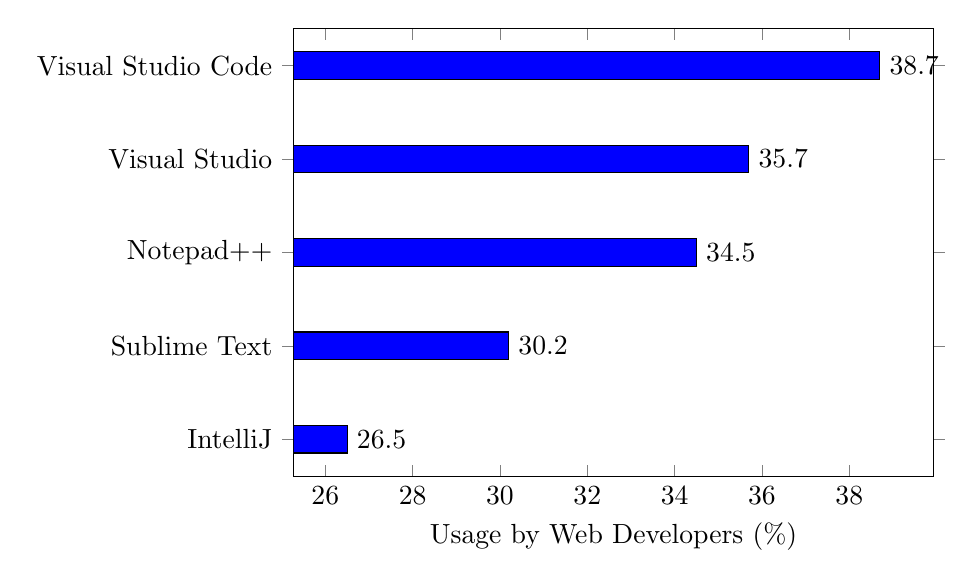
\begin{tikzpicture}
        \begin{axis}[
            symbolic y coords={IntelliJ,Sublime Text,Notepad++, Visual Studio,Visual Studio Code},
            xlabel=Usage by Web Developers (\%),
            width=0.8\textwidth,
            height=0.6\textwidth,
            xbar,
            nodes near coords,
            nodes near coords align={horizontal},
          ]
            \addplot[xbar,fill=blue] coordinates {
                (26.5,IntelliJ)
                (30.2,Sublime Text)
                (34.5,Notepad++)
                (35.7,Visual Studio)
                (38.7,Visual Studio Code)
            };
        \end{axis}
    \end{tikzpicture}
\caption[Top 5 most used IDEs by Web developers]{Top 5 most used IDEs by Web developers \footnotemark}
\label{fig:topIdes}
\end{figure}
\footnotetext{data retrieved  from https://insights.stackoverflow.com/survey/2018/}
\par


ASP.NET also offers automatic monitoring built in. This allows the maintainers to monitor the applications for some basic problems (like infinite loops or memory leaks) and immediately take action to solve the problem. This ensures the higher stability of the application \parencite{prosAndConsNetCore}.

\par


However, the support of data-oriented development for .NET (and not just .NET Core) is provided by Entity Framework. Entity Framework is an \gls{ORM} that connects the model of the application to relational databases. This framework is thought to offer low flexibility and not support all database designs. The fact of the development environment being Visual Studio also brings problems. The licensing costs of the \gls{IDE} is about \$45 per month/user for the base version\footnote{prices retrieved from https://visualstudio.microsoft.com/pt-br/vs/pricing/ on 16/02/2019}. Some people also complaint about the technology being too connected to its vendor, Microsoft \parencite{prosAndConsNetCore}. As opposed to other frameworks that are much more community-driven, .NET still depends on decisions made by Microsoft, which may lead to offer no alternatives for integration that the ones that are distributed by them.


\subsubsection{Java Spring}
\label{sub:StateOfTheArt_Frameworks_java}
Java Spring is an open-source application framework that provides core features to the Java platform. The first version of this framework was released in 2002 by Rod Johnson as a beta, reaching to a stable version in 2004. Despite being an open-source platform, it is maintained by Pivotal.

\par

Java Spring is a very flexible framework that supports both \gls{XML} and annotations for configuring the Spring Beans. The beans are the backbone of the application that are instantiated, assembled and managed by the Spring \gls{IoC}. The \gls{IoC} is "a process in which an object defines its dependencies without creating them" \parencite{whatIsASpringBean}

\par
This framework provides support for several services, like \gls{AOP} for cross-cutting concerns, Authentication and Authorization, dependency injection and testing infrastructure, to write unit and integration tests. There is also a data access framework that abstracts the developer from many common difficulties that are faced. The most common data access frameworks for Java, such as \gls{JPA} and Hibernate are also supported \parencite{springFramework}. 
\par

Spring also offers support for \gls{JDK} timers, logging frameworks and libraries that contain many useful functions for the developers to learn and use them to develop applications \parencite{prosAndConsJavaSpring}. 

\par
Being built on top of Java, this means that it will run on the \gls{JVM}. The \gls{JVM} is a virtual machine that runs on top of the \gls{OS}, abstracting its procedure calls and standardizing them for the programming language. This means that an application that was built using Java Spring, can run on any \gls{OS} \parencite{whatIsTheJVM}. This was a great advantage that Java had over its competitors, specially on the web development industry. Competitors like Microsoft's .NET didn't support cross-platform. However, in 2016, Microsoft presented .NET Core. A framework based on .NET but that could run on any machine. 
\par 
Two of the main cons of the Spring Framework are its complexity and the long learning curve. This happens due to the 2400+ classes plus tools that the developers need to know to be able to develop their applications \parencite{javaSpringAdvantagesAndDisadvantages}. This can make the project far more complex than what it needed to be. Also, there are no clear security guidelines. Cross-site scripting attacks or cross-site request forgery attacks avoidance are examples of documentation that is missing \parencite{prosAndConsJavaSpring}.

\subsubsection{Node.js}
\label{sub:StateOfTheArt_Frameworks_Node}
Node.js is a \gls{JS} runtime environment. It uses the Google Chrome V8 engine in order to run the code. As JavaScript was originally made to run in the client application, Node was born to extend the language to the back-end side \parencite{whatIsNodejs}.
\par
Node's main idea was to "use non-blocking, event-driven I/O to remain lightweight and efficient in the face of data-intensive real-time applications that run across distributed devices" \parencite{whyUseNode}. That means that this technology didn't come to overcome every problem ever faced. Instead, it solves a particular need in the development world. For example, as Node is single threaded, it is not indicated for heavy \gls{CPU} operations. The main advantage or using it is to build fast, scalable and lightweight applications. Another benefit of using Node.js is that both the front-end and back-end will be in a common language. This causes for a fast synchronization, which is especially good for event-based applications \parencite{goodAndBadOfNode}. 
\par
The way how it works is different from the traditional implementations. On that approaches, each new request would start a new thread in the system, using its \gls{RAM}. When the available memory is all in use, the new connections will stay on-hold, waiting for a thread to be available. On the other hand, Node.js uses non-blocking I/O calls, which allows it to handle "tens of thousands of concurrent connections" \parencite{whyUseNode}. The figure \ref{fig:nodeThreadManagement} demonstrates the difference between the thread management done in both the traditional applications and in Node.js.
\par


\begin{figure}[ht]
\centering
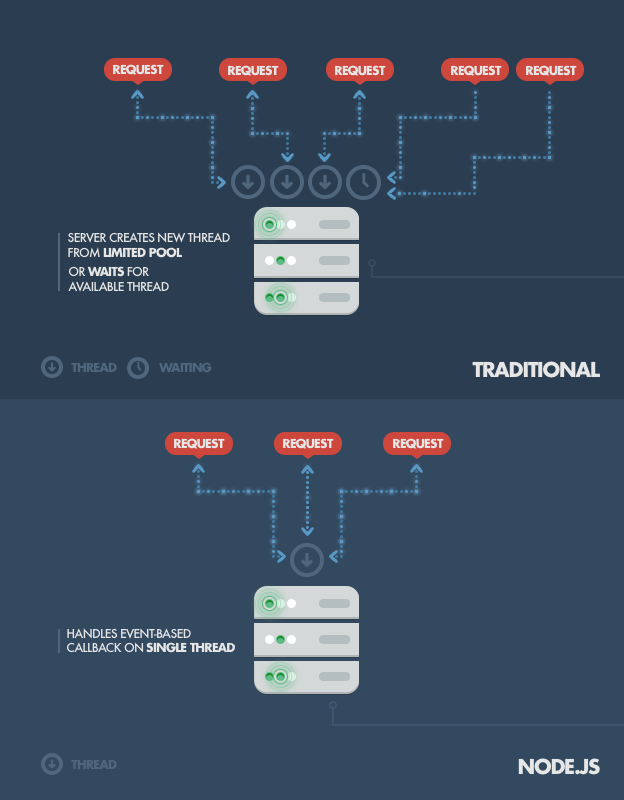
\includegraphics[width=0.8\textwidth,keepaspectratio]{chapters/State_of_the_Art/assets/node-functioning.png}
\caption[Node.js Thread management]{Node.js Thread management\footnotemark}
\label{fig:nodeThreadManagement}
\end{figure}


\par
All the points that were referred above, make Node.js as a perfect platform to be used in applications such as chat rooms, data streaming systems and stock trading platforms.
\par

As every good thing has a but, Node is no exception. Despite being a quite new technology, the core of node modules is considered stable. However, many tool on npm (the Node.js package manager) are of poor quality and/or have not being properly documented \parencite{goodAndBadOfNode}. The fact of being open-source also has an impact. Despite the core modules being supervised by Joyent and other major contributors, the rest of the tools might lack in the code quality. There are also some performance problems when working with Node. As JavaScript was made to be asynchronous, it has a non-blocking \gls{I/O} model. This means that it can process many reads and writes that are queued in the background, without blocking the main thread. For this, Node uses callbacks. Callbacks are functions that run on background in a queue. If there is a situation where callbacks are nested within other callbacks, it will make the code difficult to read a maintain. This is commonly known as callback hell. The listing \ref{lst:callback_hell} presents an example of this problem.
\footnotetext{retrieved from https://www.toptal.com/nodejs/why-the-hell-would-i-use-node-js}
\par

\begin{minipage}{\linewidth}
\lstinputlisting [caption={Callback Hell example\protect\footnotemark.},
label=lst:callback_hell]
{chapters/State_of_the_Art/assets/callback-hell.js}
\end{minipage}
\footnotetext{retrieved from http://callbackhell.com/ on 16/02/2019}

\par
 Node is constantly chosen for solutions that require real-time updated data, like video-conference systems or online gaming. By using \gls{JS} programming language, the learning curve for Node is kept to a minimum. This means that developers with front-end experience (which requires a lot of JavaScript) can start programming server-side without facing many difficulties. The fact of being a lightweight makes this a very good option for micro-service architectures. Despite being an open-source technology, it has a great corporate support. That support was initially provided by Joyent, but in 2015, with the creation of the Node.js Foundation, IBM, Microsoft, Paypal, SAP and Fidelity also offered their support by becoming founding members or the organization \parencite{goodAndBadOfNode}.
\par


\subsection{Swagger}
\label{sub:swagger}
Swagger is an open-source framework that allows the generation of automatic documentation of the available endpoints in an \gls{API}. This is done without any human intervention. Swagger is capable to ask the \gls{API} for an YAML or a JSON file that contains a detailed structure of the entire \gls{API}. This file is essentially a resource listing using the OpenAPI specification. This file contains the following information \parencite{whatIsSwagger}:
\begin{itemize}
    \item What are the operations supported by the \gls{API};
    \item What are the endpoint's parameters and return values;
    \item Authentication and Authorization information.
\end{itemize}

\begin{figure}[ht]
\centering
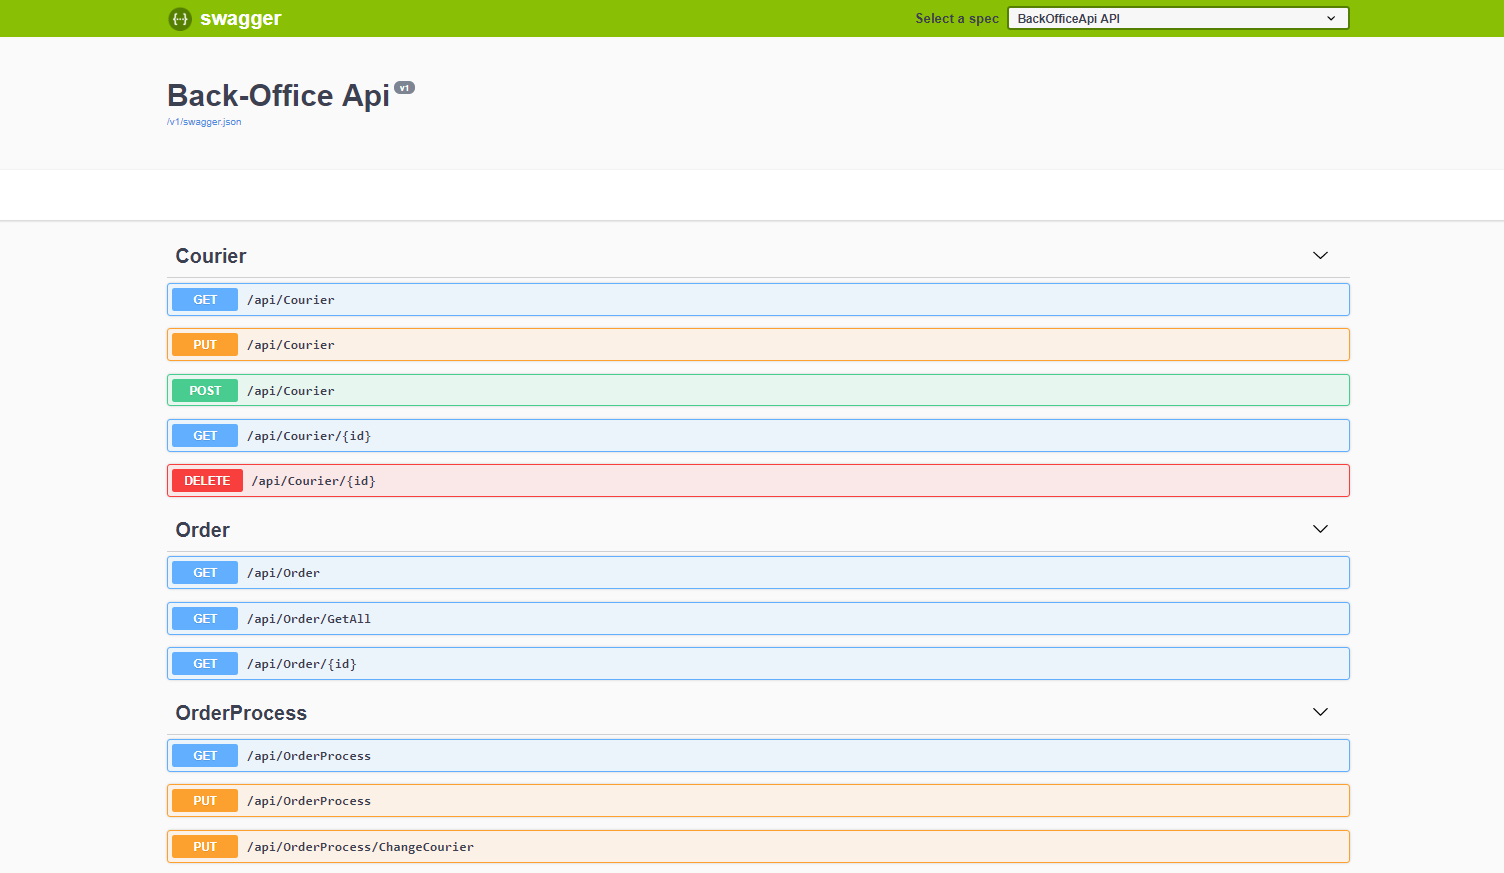
\includegraphics[width=\textwidth,keepaspectratio]{chapters/State_of_the_Art/assets/backoffice-api-endpoints.PNG}
\caption[Back-Office API Endpoints on Swagger page]{Back-Office API Endpoints on Swagger page}
\label{fig:swaggerEndpoints}
\end{figure}

\par
The figure \ref{fig:swaggerEndpoints} shows the listing of endpoints in one of the solution's \glspl{API}, Back-Office API. This allows the consumers to know from the start how to use the \gls{API}. Opening one endpoint, as shown in figure \ref{fig:endpointExample}, it is possible to verify the required parameters, the return value and even to call that endpoint, making it easier to make a direct request to the \gls{API}.

\begin{figure}[!hb]
\centering
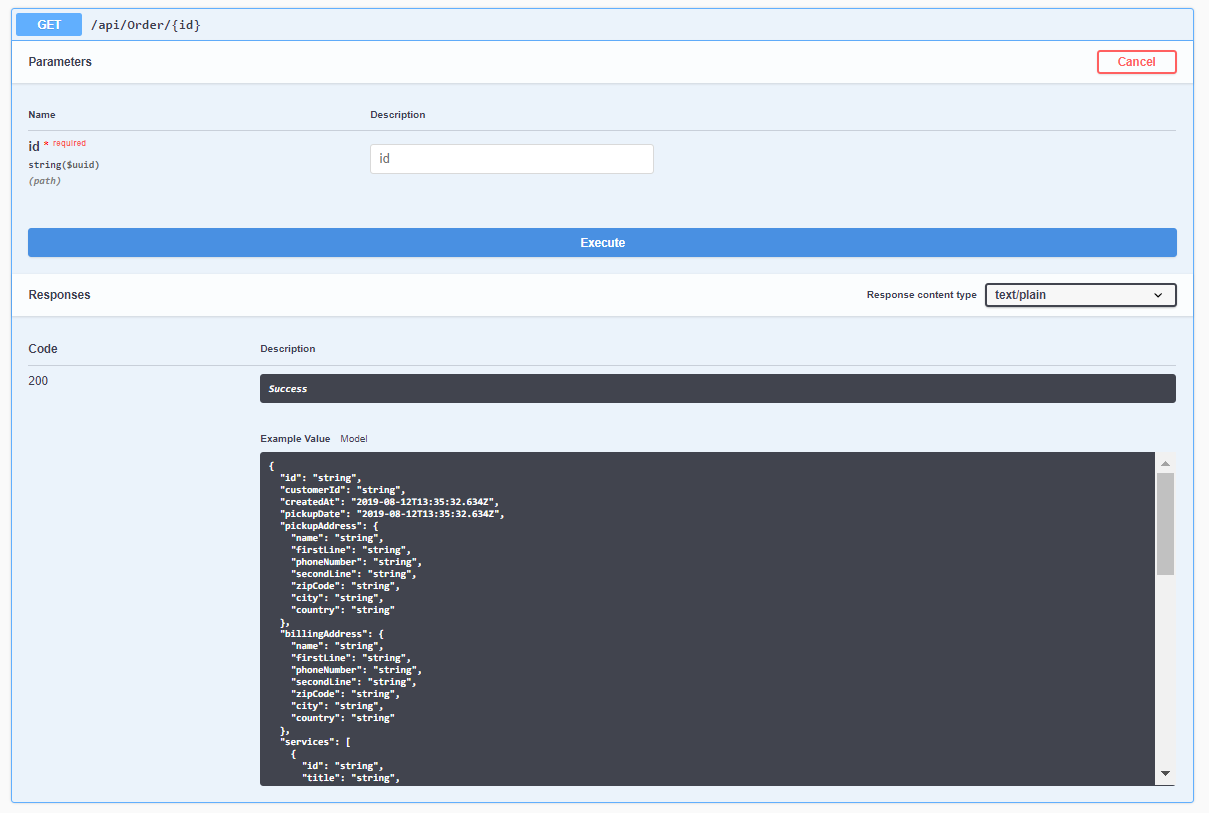
\includegraphics[width=\textwidth,keepaspectratio]{chapters/State_of_the_Art/assets/open-endpoint.PNG}
\caption[Open endpoint on Swagger]{Open endpoint on Swagger}
\label{fig:endpointExample}
\end{figure}

\par

Swagger has support for many languages and frameworks, such as .NET, Java, Go, C++, etc.
